\documentclass[a4paper,11pt]{report}

\usepackage[utf8]{inputenc}
\usepackage[english]{babel}
\usepackage[left=3cm, right=3cm, top=3cm, bottom=3cm]{geometry}
\usepackage{amsthm}
\usepackage{amsmath}
\usepackage{graphicx}
\usepackage{float}
\usepackage{caption}
\usepackage{subcaption}
\usepackage{listings}
\usepackage[dvipsnames]{xcolor}
\usepackage{fancyhdr}

%counter for goals, domains and requirements
\newcounter{goalnum}
\newcounter{domnum}
\newcounter{reqnum}
\newcounter{subreqnum}[reqnum]




\newcommand{\givespace}
    {
    \vskip 0.5cm
    \noindent
    }

\newcommand{\goal}[2]{
\refstepcounter{goalnum}
\label{g:#2}
[G\thegoalnum]\; #1
\global\expandafter\def\csname goal#2\endcsname {#1} 
}
  
\newcommand{\dom}[2]{
\refstepcounter{domnum}
\label{d:#2}
[D\thedomnum] #1
\global\expandafter\def\csname dom#2\endcsname {#1}
}

\newcommand{\req}[2]{
\refstepcounter{reqnum}
\label{r:#2}
[R\thereqnum] #1
\global\expandafter\def\csname req#2\endcsname {#1}
}

\renewcommand{\thesubreqnum}{\thereqnum.\arabic{subreqnum}}

\newcommand{\subreq}[2]{
\refstepcounter{subreqnum}
\label{sr:#2}
[R\thesubreqnum]\; #1
\global\expandafter\def\csname subreq#2\endcsname {#1}
}


% header and footer
\setlength{\headheight}{14pt}

\pagestyle{fancy}
\fancyhf{}
\lhead{\color{gray}{\small{TrackMe project by Stefano Pecchia and Edoardo Peretti}}}
\lfoot{\textcolor{gray}{\small{Copyright © 2018, Stefano Pecchia and Edoardo Peretti – All rights reserved}}}
\rfoot{\textcolor{gray}{\thepage}}
\renewcommand{\headrulewidth}{0pt}

\fancypagestyle{plain}{
	\fancyhf{}
	\lfoot{\textcolor{gray}{\small{Copyright © 2018, Stefano Pecchia and Edoardo Peretti – All rights reserved}}}
\rfoot{\textcolor{gray}{\thepage}}
}






\title{Requirements Analysis and Specification Document}
\author{Stefano Pecchia \and Edoardo Peretti}
\date{\today}

\makeatletter
\let\thetitle\@title
\let\theauthor\@author
\makeatother

\begin{document}

\begin{titlepage}
\centering

\textcolor{black}{\textbf{Politecnico di Milano}} \par
\textcolor{black}{\textbf{AA 2018/2019}} \par  \vspace{2em}

\includegraphics[scale=0.7]{resources/PolimiLogo}\par \vspace{1em}

Software Engineering 2 \par \vspace{1.5cm}
\textcolor{Blue}{\Large\textbf{TrackMe}} \par \vspace{3cm}

{\textcolor{Blue}{\textbf{\Huge{Requirements Analysis and Specification Document}}}} \vfill
\renewcommand\tabcolsep{4.5em}
\begin{tabular}{cc}
Stefano Pecchia & Edoardo Peretti   \\
921201  & 921286
\end{tabular}
\renewcommand\tabcolsep{6pt}
\vspace{4cm}
\end{titlepage}



\begin{table}[h!]
\centering
\begin{tabular}{rl}
\hline
\textbf{Deliverable:} & RASD\\
\textbf{Title:} & Requirements Analysis and Verification Document \\
\textbf{Authors:} & Stefano Pecchia and Edoardo Peretti\\
\textbf{Version:} & 1.1 \\ 
\textbf{Date:} & \today \\
\textbf{Download:} & https://github.com/Speck1996/PecchiaPeretti \\
\textbf{Copyright:} & Copyright © 2018, S. Pecchia and E. Peretti – All rights reserved \\
\hline
\end{tabular}
\end{table}



\tableofcontents


%chapters

\chapter{Introduction}
\section{Purpose}

\textbf{Data4Help} is a service whose aim is to collect eHealth data acquired from registered users and make it available for other particular users, called third parties.

\par \noindent \newline
The purpose of this document is to give an overview of Data4Help capabilities, serving as a guideline to fully understand what this system should provide to the end users. Reading this report
is essential to gather all the information needed for the software developing and testing, especially to distinguish  \textbf{what is assumed by the system} and what is \textbf{required} from it.

\par \noindent \newline
Data4Help is a system that can allow the joining of two typologies of users:
\begin{itemize}
\item Individuals that want their data to be acquired by Data4Help.
\item Third-Parties that want to access the collected data.
\end{itemize}
The system should also provide another service, built on top of Data4Help, called AutomatedSOS.
\newline
 This service monitors the health status of the subscribed user and when some parameters are below certain thresholds, sends to the customer and ambulance.
\newline
Improving users lifestyle and helping third party to analyze their health status will be the key driver of Data4Help features.
\newline
In the following chapters more details will be presented.


\section{Scope}
\subsection{Description of the given problem}
Data4Help aims to collect and gather in one place all the data related to the health condition of a registered user (steps taken daily, average heart beat, possible activities done in a day) from any device capable of collecting at least one of these kind of data.
The collected data can be accessed by third-parties in two different ways:
\begin{itemize}
\item Anonymized data: data of group of individuals, where the group can be identified by location, parameters on specific data (both on the user and the collected data). To maintain a certain level of privacy requests that select groups that count higher than 1000 individuals are allowed by the system.
\item Specific individual data: data of a specific user, this can be accessed only after the third-party sends a request to access the user data, and the user accepts it. The handling of the request for individual data is handled by the system.
\end{itemize}
The system also updates as soon as possible the third parties, when new accessible data is gathered.
To distinguish between individuals account, and third parties account at the moment of registration the user must select what kind of account it is going to create.
Third parties can also subscribe to another service, included in the application: AutomatedSOS. This service monitors the health status of an individual continuously, and, if certain parameters go below a critical threshold, the application starts automatically a rescue procedure. The rescue procedure should start in under 5 seconds from the crossing of the treshold and consists in sending an ambulance to the position of the user.
\newline
In a fragmented market like the wearables one, Data4Help focus on organizing all the data coming these devices and provide it easily while respecting user privacy.
 \newline
This is not the only purpose of Data4Help, indeed the AutomatedSOS service enable the system to have an active role in the life of its users, monitoring their health constatly and providing them emergency support.
\subsection{World and machine phenomena}
\begin{figure}
\centering
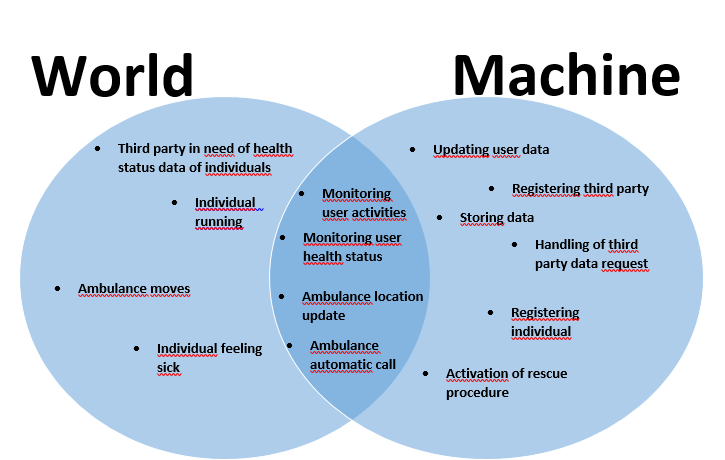
\includegraphics[scale=0.7]{img/phenomena.png}
\end{figure}


\subsection{Goals}

\begin{goal}
The users' eHealth data are correctly gathered from their device and uploaded to the system.
\end{goal}
\begin{goal}
Registered third-parties can access anonimized data.
\end{goal}
\begin{goal}
A registered third party can ask for permission to access an individual data.
\end{goal}
\begin{goal}
A registered third party can access the data of an individual who gave permission to it
\end{goal}
\begin{goal}
The system is able to start automatically a rescue procedure.
\end{goal}
\begin{goal}
The system is able to mantain the desired privacy level of each user (?).
\end{goal}
\begin{goal}
The system updates the third-party when new data of accepted requests is available
\end{goal}
\section{Definitions, Acronyms, Abbreviations}
\subsection{Definitions}
\begin{itemize}
\item \textbf{Rescue Procedure}: all the operations needed to save a person life. The operations include both the ones handled by computers and humans.
\item \textbf{eHealth Data}: all the data that can the related to the general health of the user, for example steps taken daily, hearth beat, blood pressure, activity level
\item \textbf{Health status}: level of health of a person, obtained analyzing various parameters like  hearthbeat rate, weight, hours of sleep.
\item \textbf{Critical Treshold}: value that, referred to an health parameter, must not be passed to guarantee user vital activities.
\end{itemize}




\subsection{Acronyms}

\begin{itemize}
\item \textbf{SSN}: Social Security Number
\item \textbf{TC}: Tax Code
\end{itemize}




\section{Revision History}
\section{Reference Documents}
\section{Document Structure}
\chapter{Overall description}
\section{Product perspective}
Data4Help is a brand new service that will be built from the ground up. The user will interact with the system through the mobile application. An internet connection, GPS, and a wearable to collect eHealth data are required in order to use Data4Help fuctionalities and the optional additional service AutomatedSOS.
\section{Product functions}


\subsection{Access to specific data}
A third party interested in monitoring a specific individual can send a request to the system specifying his SSN or TC.
The system passes the request to the specific individual who can accept or refuse it.
If the request is accepted, the third party can see daily or aggregate data of the individual. In this case the third party can also see name, surname and age of the individuals.


\subsection{Access to group data}
A third party can also request access to anonymized data of a group of individuals.
To do so, it must specify some parameters concerning individuals. These parameters can regard geographical area, age range or level of education of the users of interest to the third party.
Geographical area can be specified in term of country, region, province, town and district (only for big city).

This type of requests are managed directly by the system. Because TrackMe holds in high regard the privacy of its users, it will satisfy the request only if the number of individuals whose data satisfy the request is higher than 1000.

If the request is positively evaluated, the anonymized data is made available to the third party.
Optionally, the third party can subscribe to new data with the same characteristics. If new data, matching the third party request, is produced it will be made available to the requester at most once a week.




\subsection{SOS service}
The service AutomatedSOS must exploit the real-time stream of eHealth data provided by the underlying Data4Help to offer a personalized and non-intrusive SOS service especially designed for elderly people.
Any individual, correctly registered to Data4Help, can optionally request to active this service


If AutomatedSOS has been activated, the system should continuously monitor the parameters of the individuals and compare them using certain specific thresholds.
If the parameters are below these thresholds, the system assumes that the individual is having a sudden illness and forwards a request to an emergency service for sending an ambulance to the location of the user.
AutomatedSOS must ensure a reaction time of less than 5 seconds from the time the parameters are detected below the threshold.










\section{User characteristics}
The users of Data4Help and AutomatedSOS services are:

\begin{itemize}
\item \textit{Individual} : user that allows the acquisition of the data and can optionally activate AutomatedSOS. He can't use the data request feature of Data4Help.
\item \textit{Third party}: user that can request data from the application.
\end{itemize}





\section{Assumptions, dependencies and constraints}

\subsection{Domain assumptions}

\begin{itemize}


\item[]\dom{ 
Location and eHealth data are provided by individuals' devices and assumed to be correct.
}{•} 
\item[]\dom{
A third party interested in monitoring a specific individual knows the SSN of the individual
}{•}
\item[]\dom{
Users have access to internet.
}{•}
\item[]\dom{
Thresholds for health parameters are provided by medical experts.
}{•}
\item[]\dom{
An ambulance is always available when it is needed.
}{•}
\item[]\dom{
Registered users must keep their login credentials secret.
}{•}
\item[]\dom{
The ambulance driver can reach the user in critical condition.
}{•}
\end{itemize}




\subsection{Privacy constraints}
The system will collect and elaborate personal data of the individuals and, possibly, it will share them or part of them with third party.  For this reason, during the registration activity to the system, all the users must be informed of this practice and they must explicitly confirm their consensus.

In particular, anonymized data can be shared with third parties who request it without the users being further advised. In order to protect its users' privacy and to prevent misuse of data, TrackMe won't share data if the number of individuals whose data satisfy the request is lower than 1000.

Moreover, a third party can request to fully access the data of some specific individual. In this case it is up to the individual to accept or not to share his data with that specific third party.

\subsection{Hardware limitations}
These are the devices that will first receive Data4Help app. 
In the future other smartwatch operating systems may be considered.
\begin{itemize}
\item iOS or Android smartphone with following capabilities:
\begin{itemize}
\item 2G/3G/4G connection
\item GPS
\end{itemize}
\item watchOS or wearOS smartwatch
\end{itemize}


\chapter{Specific requirements}

\section{External Interface Requirements}


\subsection{Hardware Interfaces}
Data4Help is a software application, therefore no hardware interface is needed. However the application needs a smartphone with working bluetooth and internet in order to guarantee its primary services (collecting and updating eHealth data from user devices). 
In addition, the AutomatedSOS service requires that the users' smartphone has location services enabled.


\subsection{Software Interfaces}
In order to guarantee a quick development Data4Help system will use the following external services:
\begin{itemize}
\item DataBase engine : this service will be used to manage all users data and satisfy third party queries
\item Map: individuals with AutomatedSOS service will be able to see the live position of their ambulance whenever a rescue procedure is activated.
\end{itemize}

\section{Scenarios}
\subsection{Scenario 1}

Rebecca has worked very hard in the last months and she has been a long stressful periods. Recently she had to skip several working days because she didn't feel very well. 
She consulted her doctor John who didn't notice anything alarming.
John recently discovered Data4Help and he thinks that it could be useful to monitor the health status of Rebecca on daily basis for the next weeks.
Then, John asked Rebecca to register to Data4Help and to use her smartwatch to collect some data.
Rebecca immediately registered to the service and accepted the request that John sent to her.
Now John can have a better look at his patient's health status and can make better diagnosis.


\subsection{Scenario 2}
Walter is a 75 years old man who lives alone in a small town.
His doctor has been monitoring him thanks to Data4Help because he has a cardiac disease.
Last week, Walter was at the supermarket and suddenly he fainted. Luckily, the store was crowded and therefore someone helped him and called an ambulance.
He is afraid it could happen again and because he lives alone, he decides to activate the AutomatedSOS service.


\subsection{Scenario 3}
FatBit is a startup that wants to launch its first wearable. To optimize their limited resources and to improve their ads, Fatbit's managers want to know wich are the countries with healtier people,wich one have the more active, and the average age of their potential consumers. Collecting this data it's not easy, especially when joining the market for the first time. Fortunately a new service, Data4Help, has just launched and one of its main features it's the distribution of eHealth data, organized according to different parameters, included the ones FatBit managers are interested in (age,location,steps taken daily).
Therefore FatBit's managers decide to register with a unique account as third-party, and start their data analysis thanks to Data4Help.


\subsection{Scenario 4}
Wile is an engineering student who wants to get back in shape. He decides to join the gym and to buy a wearable to see its progress over time. Initially Wile is satisfied by his wearable and the built in application but later he starts noticing that more and more wearables with improved design and many new features are launching in the market. Wisely, he notice that the built in application collects the data only for the producer's devices and so if he wanted to change his wearable without losing data he were pratically forced to buy a new watch from the same company. Therefore he decides to use Data4Help, allowing him to change his wearable with the one he likes the most without losing data.


\chapter{Formal analysis using Alloy}
It can be useful have a formal model for some of the main functionalities of Data4Help and AutomatedSOS. The following Alloy model explains in details the three core features of the system:

\begin{itemize}
\item The sending of an ambulance whenever the vital parameters of an individual, who has activated AutomatedSOS, crosses the given threshold. In particular, it is modelled the maximum reaction time.
\item The possibility that a third party can monitor the data of a specific individual. In particular, the model focuses on the fact that the individual must give permission to the third party in order to access his data.
\item The access to a collection of data by a third party. In particular, the systems must enforce a certain level of privacy.
\end{itemize}
For simplicity and without any loss of generality, all the entities that have a numeric value are represented with integer values in small intervals. Moreover, only upper thresholds for vital parameters are considered.

\section{Alloy model}

\definecolor{comment}{rgb}{0,0.6,0}
\definecolor{keyw}{rgb}{0,0,0.82}
\definecolor{num}{rgb}{0.5,0.5,0.5}
\definecolor{back}{rgb}{0.95,0.95,0.95}

\lstset{
backgroundcolor = \color{back},
morecomment=[l]{--},
morecomment=[s]{/*}{*/},
commentstyle = \color{comment},
morekeywords=[1]{open, sig, fact, one, Int, lone, set, some, extends, all, in, no, disj, and, or, implies, assert, check , run, pred, for},
keywordstyle = [1]{\color{keyw}},
basicstyle = \ttfamily,
frame=single,
breakatwhitespace = true,
breaklines = true,
rulecolor = \color{black},
tabsize = 3,
numbers = left,
numberstyle = \small\color{num},
literate=*
    {0}{{{\textcolor{red}0}}}1
    {1}{{{\textcolor{red}1}}}1
    {2}{{{\textcolor{red}2}}}1
    {3}{{{\textcolor{red}3}}}1
    {4}{{{\textcolor{red}4}}}1
    {5}{{{\textcolor{red}5}}}1
    {6}{{{\textcolor{red}6}}}1
    {7}{{{\textcolor{red}7}}}1
    {8}{{{\textcolor{red}8}}}1
    {9}{{{\textcolor{red}9}}}1,
    escapeinside={!}{!},
}

\begin{lstlisting}
open util/integer
open util/boolean

sig Location {
	coordX: one Int,
	coordY: one Int
}
{coordX >= -3 and coordX <= 3 and coordY >= -6 and coordY <= 6}

sig Time {
	time: one Int
}
{time >= 0 and time <= 6}

sig Individual {
	hasSOS: one Bool,
	data: lone EHealthData,
	location: lone Location,
	illness: lone Illness
}

sig EHealthData {
	heartRate: lone Int,
	bloodPressure: lone Int,
	steps: lone Int,
	sleepTime: lone Int	
}
{heartRate >= 0 and heartRate <= 6 and bloodPressure >= 0 and bloodPressure <= 6 and steps >= 0 and steps <= 6 and sleepTime >= 0 and sleepTime <= 6}

sig Illness {
	startTime: one Time
}

sig Ambulance {
	startTime: one Time,
	rescuee: one Individual,
	location: one Location
}

sig EHealthDataGroup {
	data: some EHealthData 
}

sig ThirdParty {
	request: set Request,
	monitor: set Individual,
	groupData: set EHealthDataGroup
}

abstract sig Request {
	approved: one Bool
}

sig GroupRequest extends Request {
	groupData: one EHealthDataGroup
}

sig SpecificRequest extends Request {
	individual: one Individual
}



/*
	Ambulance sending
*/

-- Every EHealthData belongs to a single Individual
fact DataBelongsToSingleIndividual {
	(all d: EHealthData | one i: Individual | i.data = d) 
}

-- There is a Ilness iff threshold have been crossed
fact IllnessIndividual{
	(all i: Individual | i.hasSOS = True and (i.data.heartRate >= 5 or i.data.bloodPressure >= 5) implies one il: Illness | il = i.illness) and	(all il: Illness | one i: Individual | il = i.illness and i.hasSOS = True and (i.data.heartRate >= 5 or i.data.bloodPressure >= 5))
}

-- Prevent two individual with same Illness
fact IllnessSigleIndividual {
	all il: Illness | no disj !i1!, !i2!: Individual | il = !i1!.illness and il = i!2!.illness
}

-- An ambulance is sent for a good reason with a reaction time of less than 2
fact AmbulanceIndividual {
	all a: Ambulance | a.rescuee.location = a.location and #a.rescuee.illness = 1 and a.startTime.time >= a.rescuee.illness.startTime.time and minus[a.startTime.time, a.rescuee.illness.startTime.time] <= 2
}

-- If an Individual is having an illness and he hade activate AutomatedSOS then an Ambulance is directed to his location.
-- Constraint also that only one ambulance has been sent
fact IndividualAmbulance {
	all i: Individual | #i.illness = 1 implies one a: Ambulance | a.rescuee = i
}



/*
	Requests
*/

-- Every request has been sent by a single ThirdParty
fact RequestThirdParty {
	(all r: Request | one t: ThirdParty | r in t.request ) 
}


/* Specific Requests */

-- A third party monitor only individuals who has accepted to be monitored
fact IndividualMonitored {
	all t: ThirdParty | all i: Individual | i in t.monitor implies 		one r: SpecificRequest | i = r.individual and r.approved = True and r in t.request
}

-- If a SpecificRequest is approved, a ThirdParty is monitoring the specific Individual
fact SpecificRequestApproved {
	all t: ThirdParty | all r: SpecificRequest | r in t.request and r.approved = True implies r.individual in t.monitor
}

-- No multiple SpecificRequest for the same Individual from the same ThirdParty
fact NoMultipleSpecificRequest {
	all t: ThirdParty | no disj r!1!, r!2!: SpecificRequest | r!1! in t.request and r!2! in t.request and r!1!.individual = r!2!.individual
}


/* Group Requests */

-- If TrackMe can properly anonymized those a EHealthDataGroup, a GroupRequest to this group is automatically accepted
fact GroupDataPrivacy {
	all r: GroupRequest | #r.groupData.data > 3 implies r.approved = True else r.approved = False
}

-- If a ThirdParty have access to a group of data then there is an approved request for them
fact GroupDataRequest {
	all t: ThirdParty | all g: EHealthDataGroup | g in t.groupData implies (one r: GroupRequest | r in t.request and r.groupData = g and r.approved = True)
}

-- If a GroupRequest is accepted, then the ThirdParty have access to EHealthDataGroup
fact {
	all t: ThirdParty | all r: GroupRequest | r in t.request and r.approved = True implies r.groupData in t.groupData
}

-- No multiple GroupRequest for the same group from the same ThirdParty
fact {
	all t: ThirdParty | no disj r!1!, r!2!: GroupRequest | r!1! in t.request and r!2! in t.request and r!1!.groupData = r!2!.groupData
}




pred ambulanceWorld {
	some i: Individual | #i.illness > 0 and some a: Ambulance | a.rescuee = i and a.startTime.time > i.illness.startTime.time
}

run ambulanceWorld for 4 but 1 Ambulance, 1 Individual, 1 Illness, 5 Int


pred groupRequestWorld {
	some r!1!, r!2!: GroupRequest | r!1!.approved = True and r!2!.approved = False
}

run groupRequestWorld for 6 but 2 Request, 1 ThirdParty, 5 Int


pred specificRequestWorld {
	some r!1!, r!2!: SpecificRequest | r!1!.approved = True and r!2!.approved = False
}

run specificRequestWorld for 5 but 2 Request, 2 Individual, 1 ThirdParty, 2 EHealthData, 0 EHealthDataGroup, 5 Int

assert privacyMaintained {
	no d: EHealthDataGroup | some t: ThirdParty | d in t.groupData and #d.data <= 3
}

check privacyMaintained for 15

assert monitorAccepted {
	no i: Individual | some t: ThirdParty | i in t.monitor and no r: SpecificRequest | r.approved = True and r in t.request
}

check monitorAccepted for 15

assert ambulanceCalling {
	no i: Individual | #i.illness > 0 and no a: Ambulance | a.rescuee = i and a.location = i.location
}

check ambulanceCalling for 15

assert ambulanceReactionTime {
	no i: Individual | #i.illness > 0 and some a: Ambulance | a.rescuee = i and a.location = i.location and minus[a.startTime.time, a.rescuee.illness.startTime.time] > 2
}

check ambulanceReactionTime for 15
\end{lstlisting}




\section{Worlds generated}

\subsection{Ambulance}
In Figure \ref{f:ambWorld}, it is shown that an ambulance is sent to the location of an Individual that he doesn't feel good.
Note that it can be there a (bounded) delay between the moment in which the vital parameters cross the thresholds (start of the Illness) and the time in which the ambulance is alerted.
\begin{lstlisting}[numbers=none]
run ambulanceWorld for 4 but 1 Ambulance, 1 Individual, 1 Illness, 5 Int
\end{lstlisting}

\begin{figure}[H]
\centering
\fbox{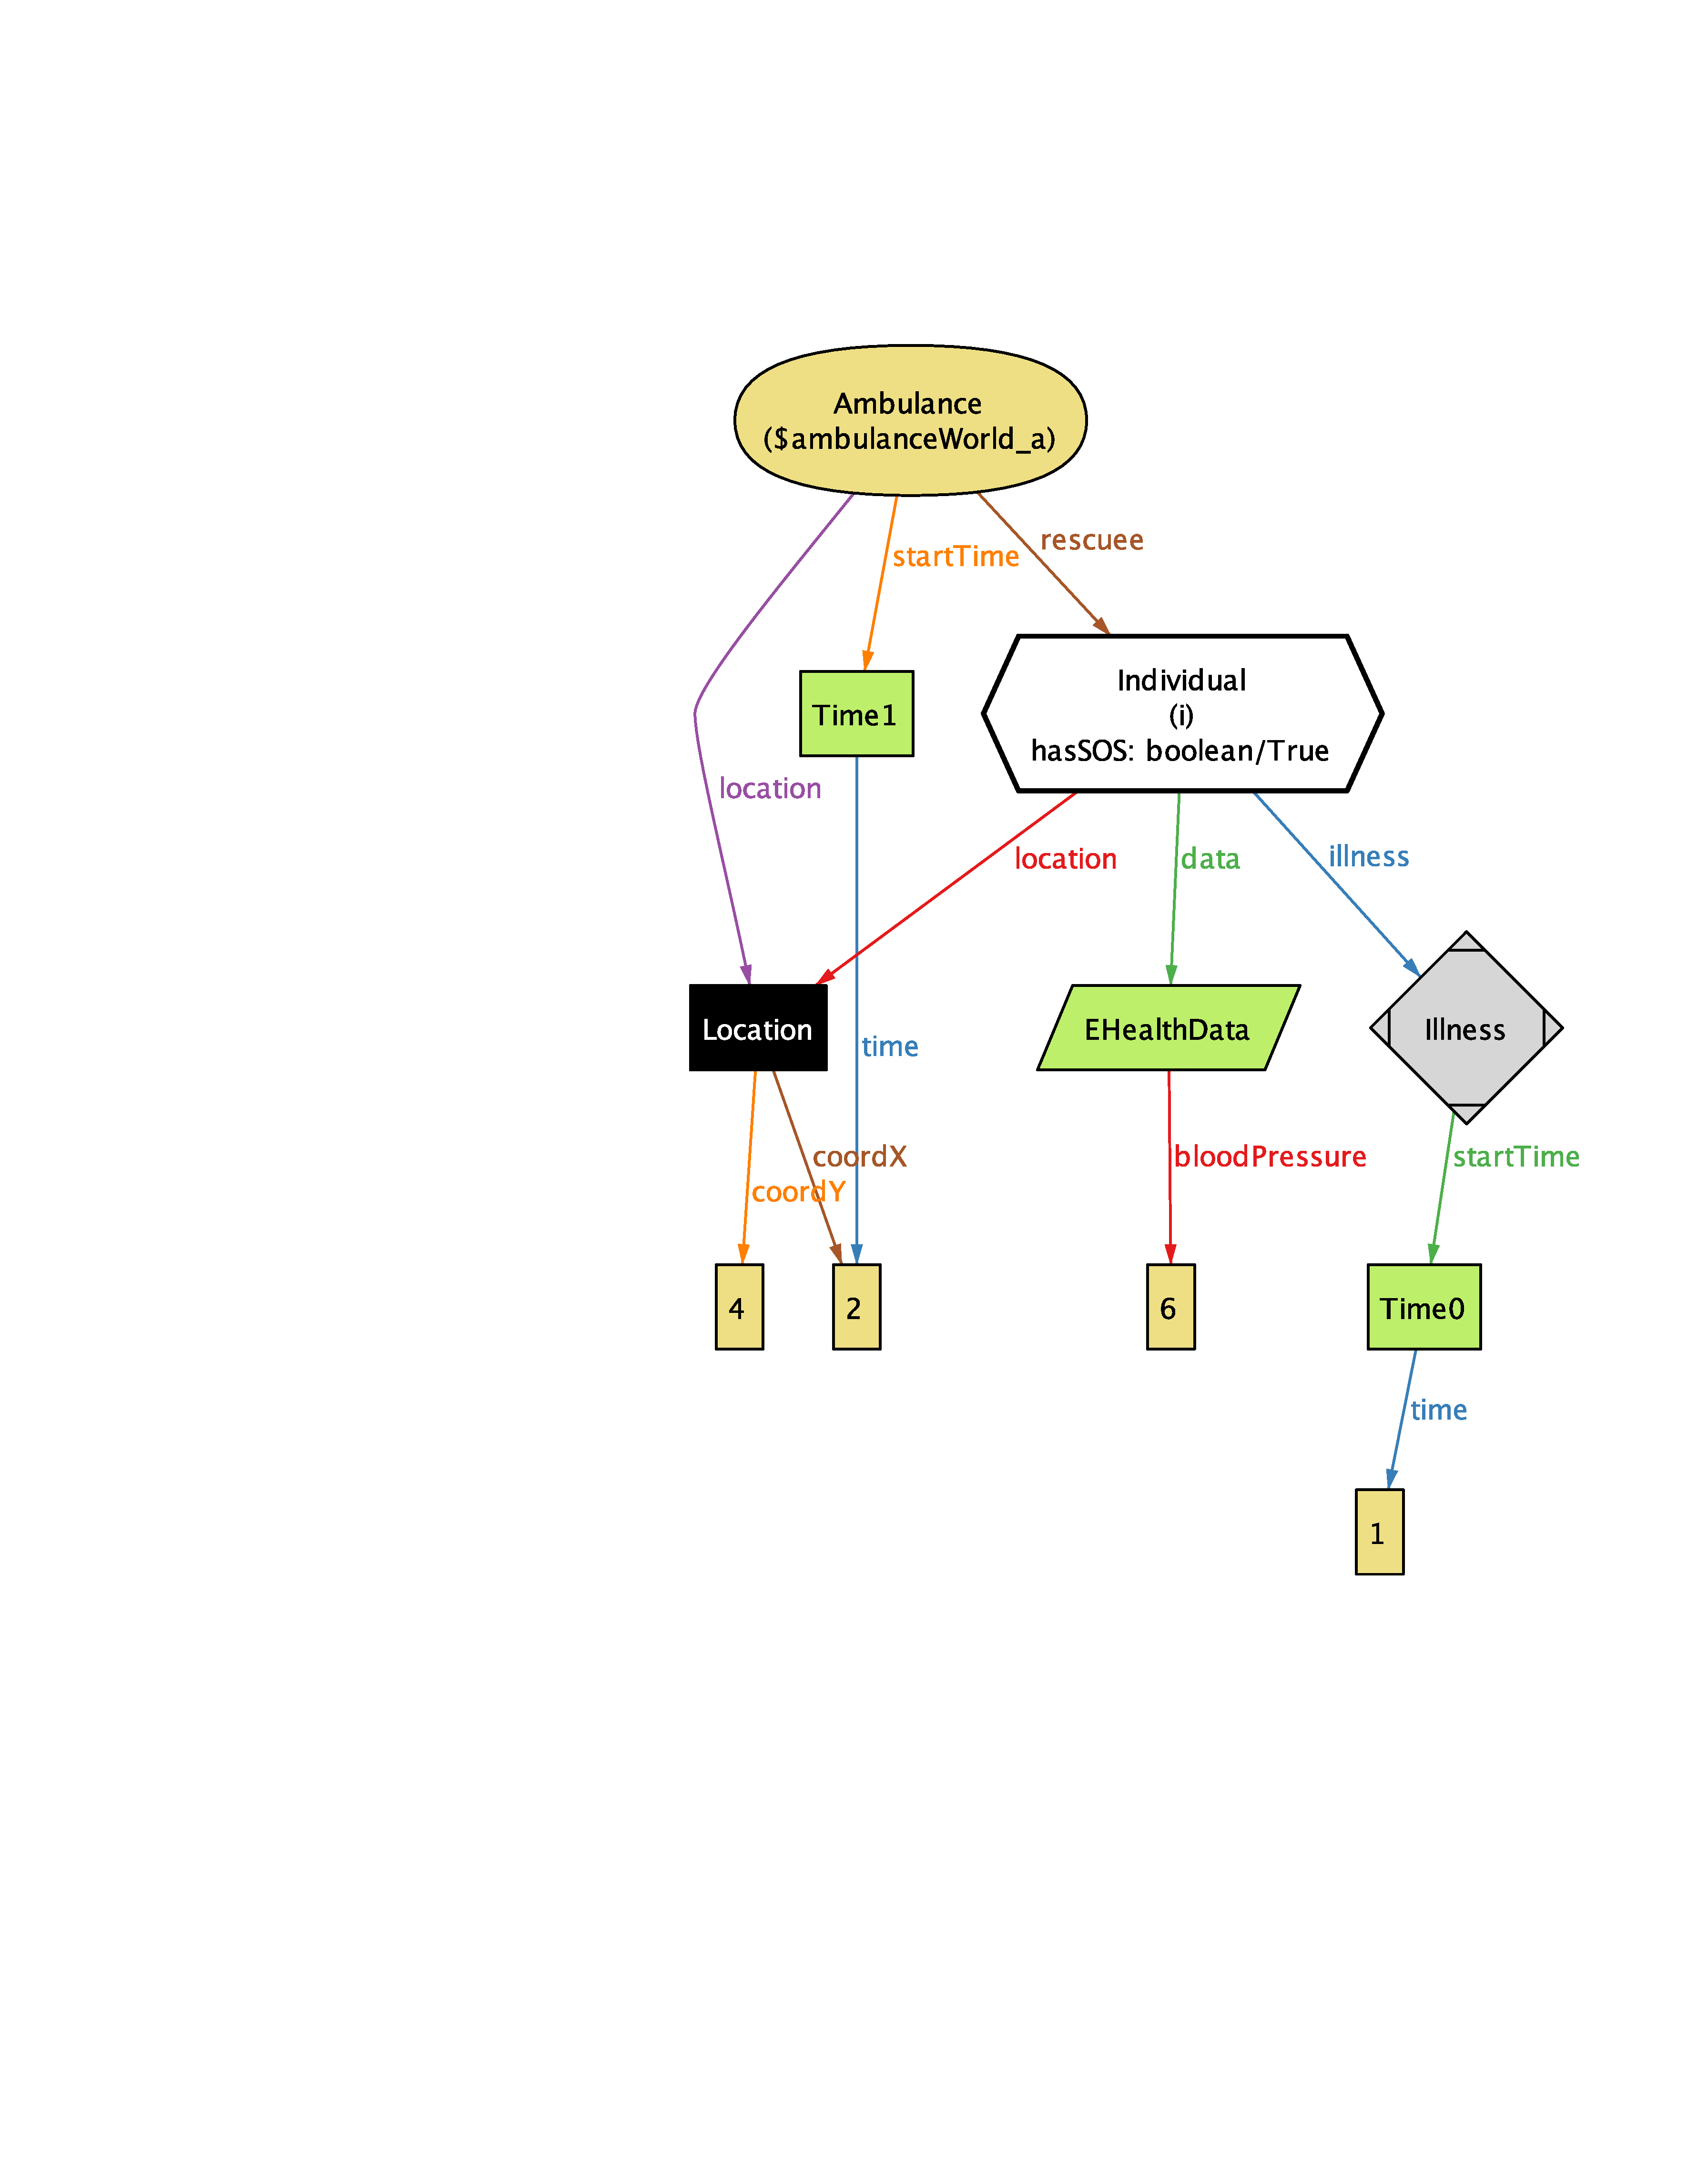
\includegraphics[width=0.9\linewidth]{resources/Alloy/ambulance}}
\caption{World generated by \texttt{ambulanceWorld} predicate}\label{f:ambWorld}
\end{figure}

\subsection{Specific requests}
In Figure \ref{f:specWorld}, it is shown a case in which a third party had sent two distinct specific request but only one is being accepted. 
Note that the third party can effectively monitor only the individual who has accepted the requests.

\begin{lstlisting}[numbers=none]
run specificRequestWorld for 5 but 2 Request, 2 Individual, 1 ThirdParty, 2 EHealthData, 0 EHealthDataGroup, 5 Int
\end{lstlisting}

\begin{figure}[H]
\centering
\fbox{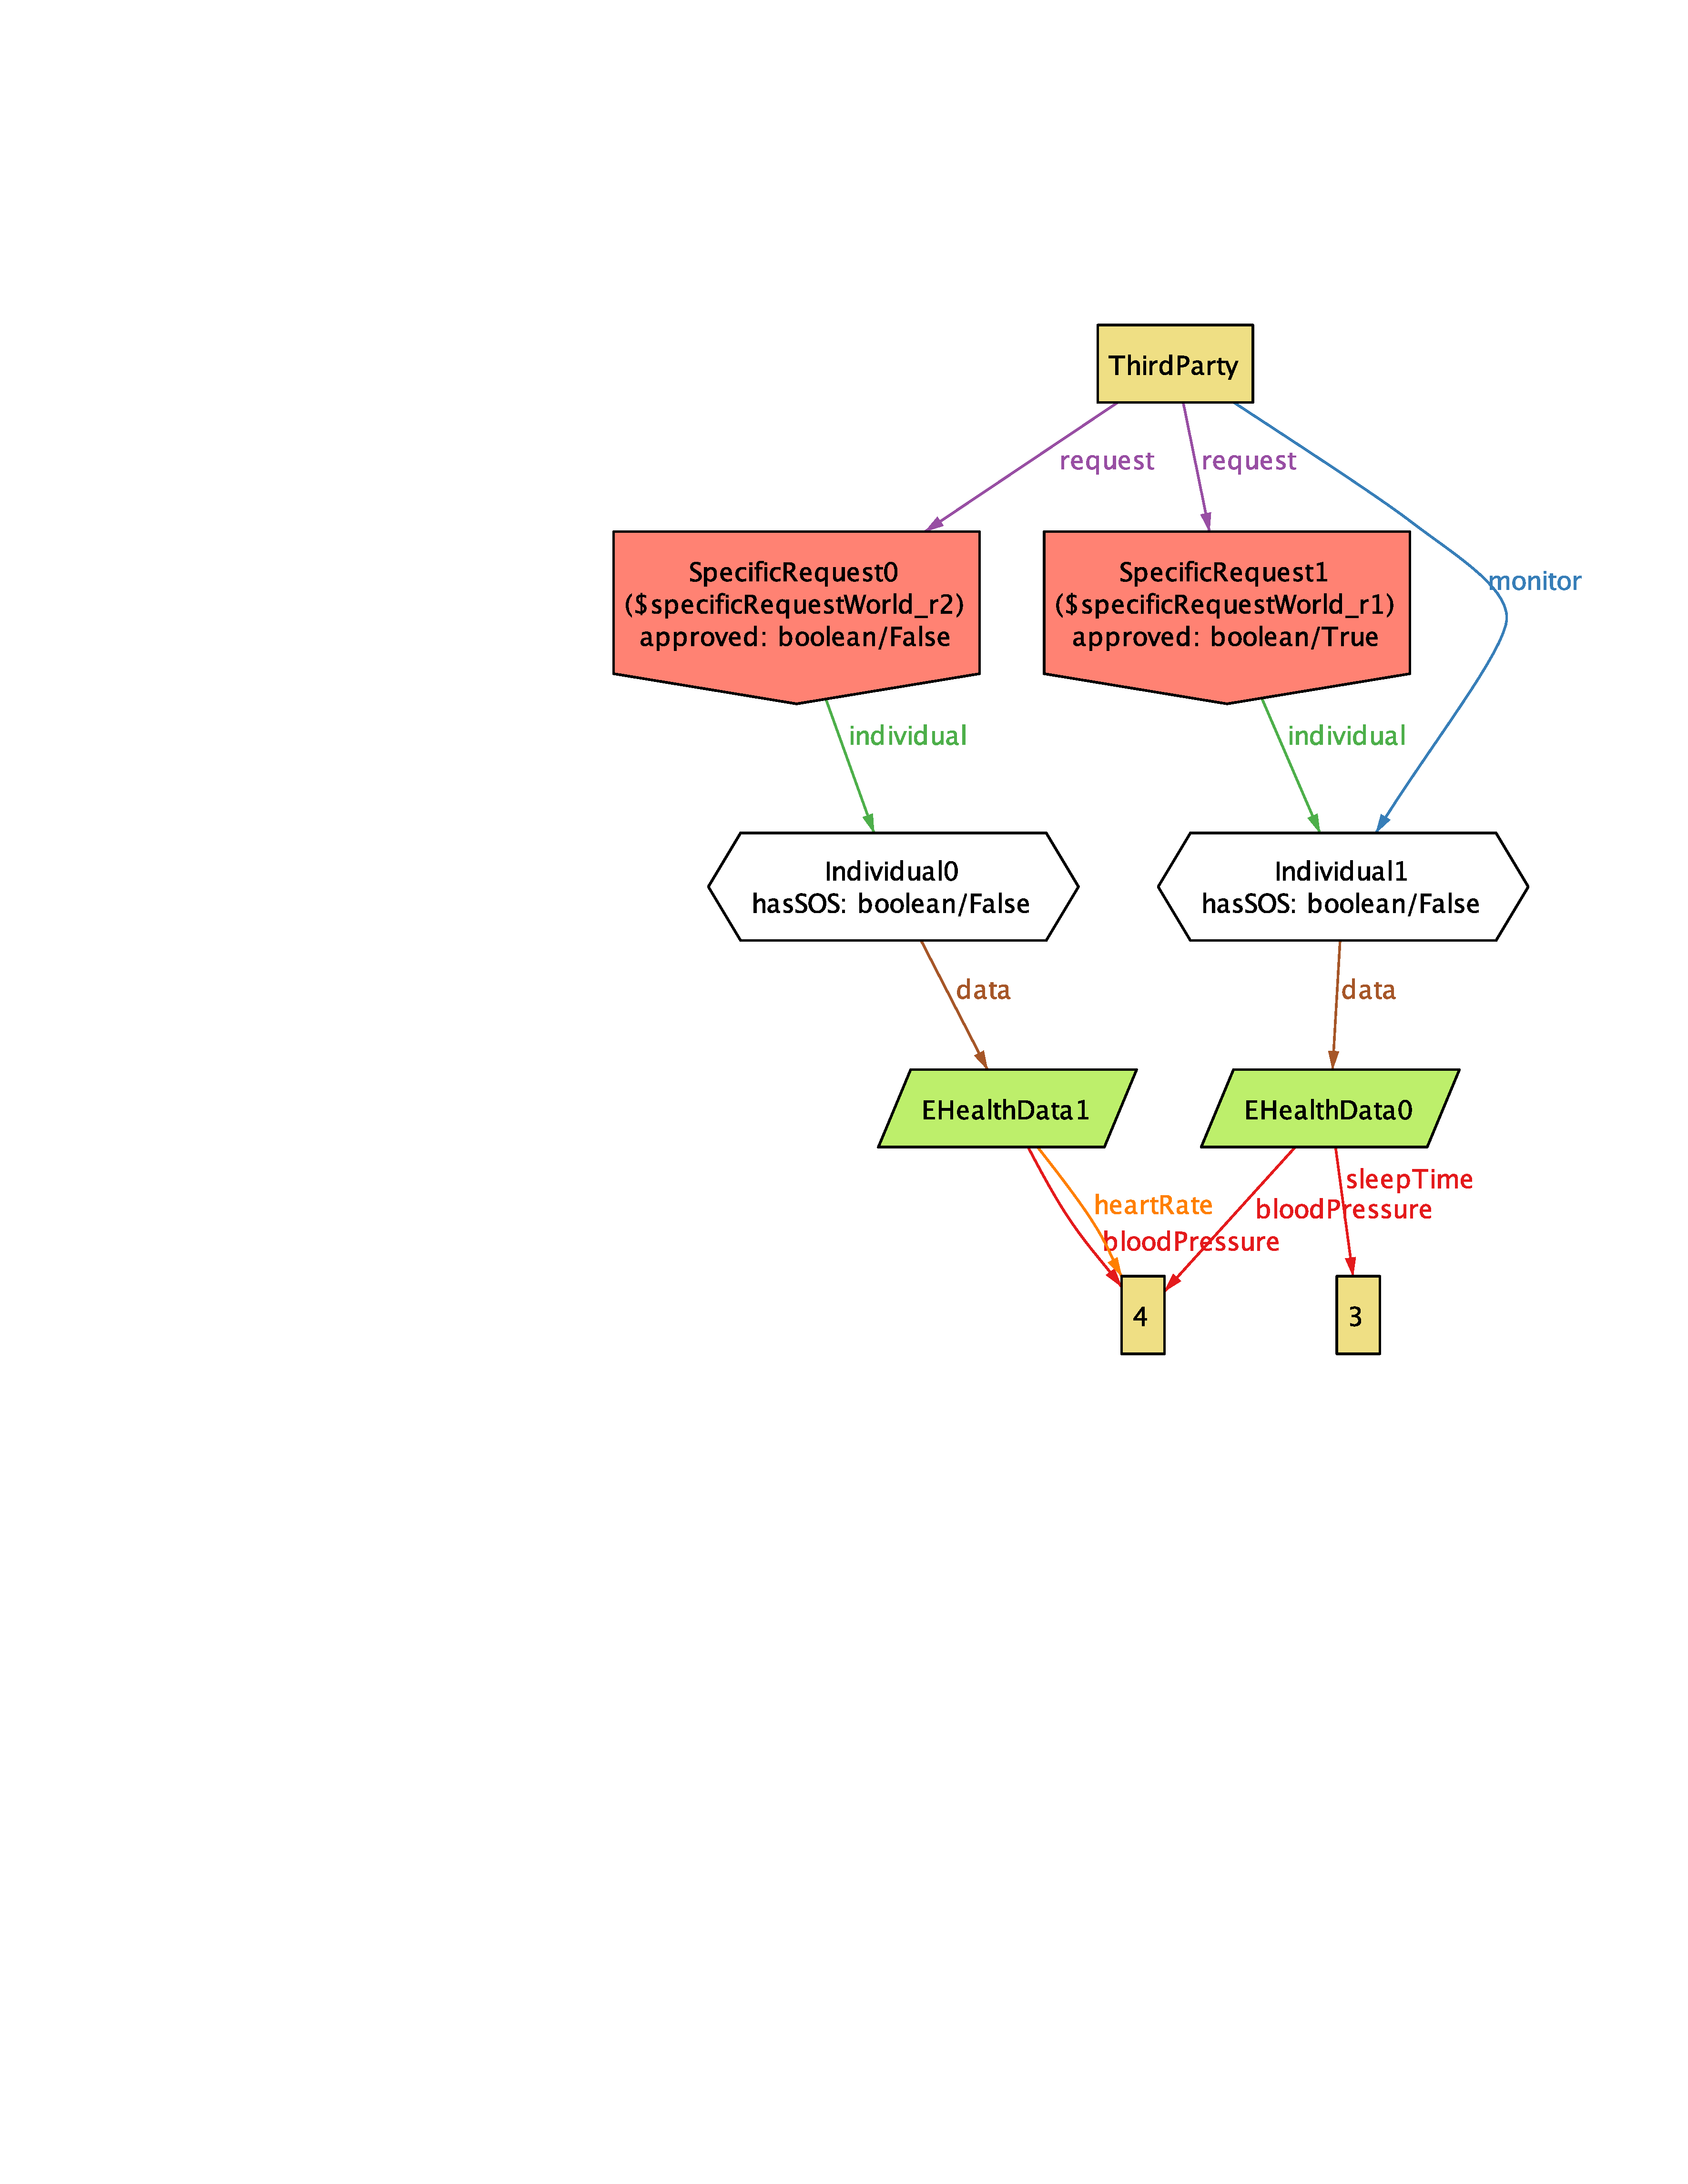
\includegraphics[scale=0.4]{resources/Alloy/specific}}
\caption{World generated by \texttt{specificRequestWorld} predicate}\label{f:specWorld}
\end{figure}


\subsection{Group requests}
Similarly to the previous, Figure \ref{f:groupWorld} shows a third party that had forwarded two group data requests. 
Note that only one respect the privacy constraint and therefore the third party can access only to one group data.
\begin{lstlisting}[numbers=none]
run groupRequestWorld for 6 but 2 Request, 1 ThirdParty, 5 Int
\end{lstlisting}

\begin{figure}[H]
\centering
\fbox{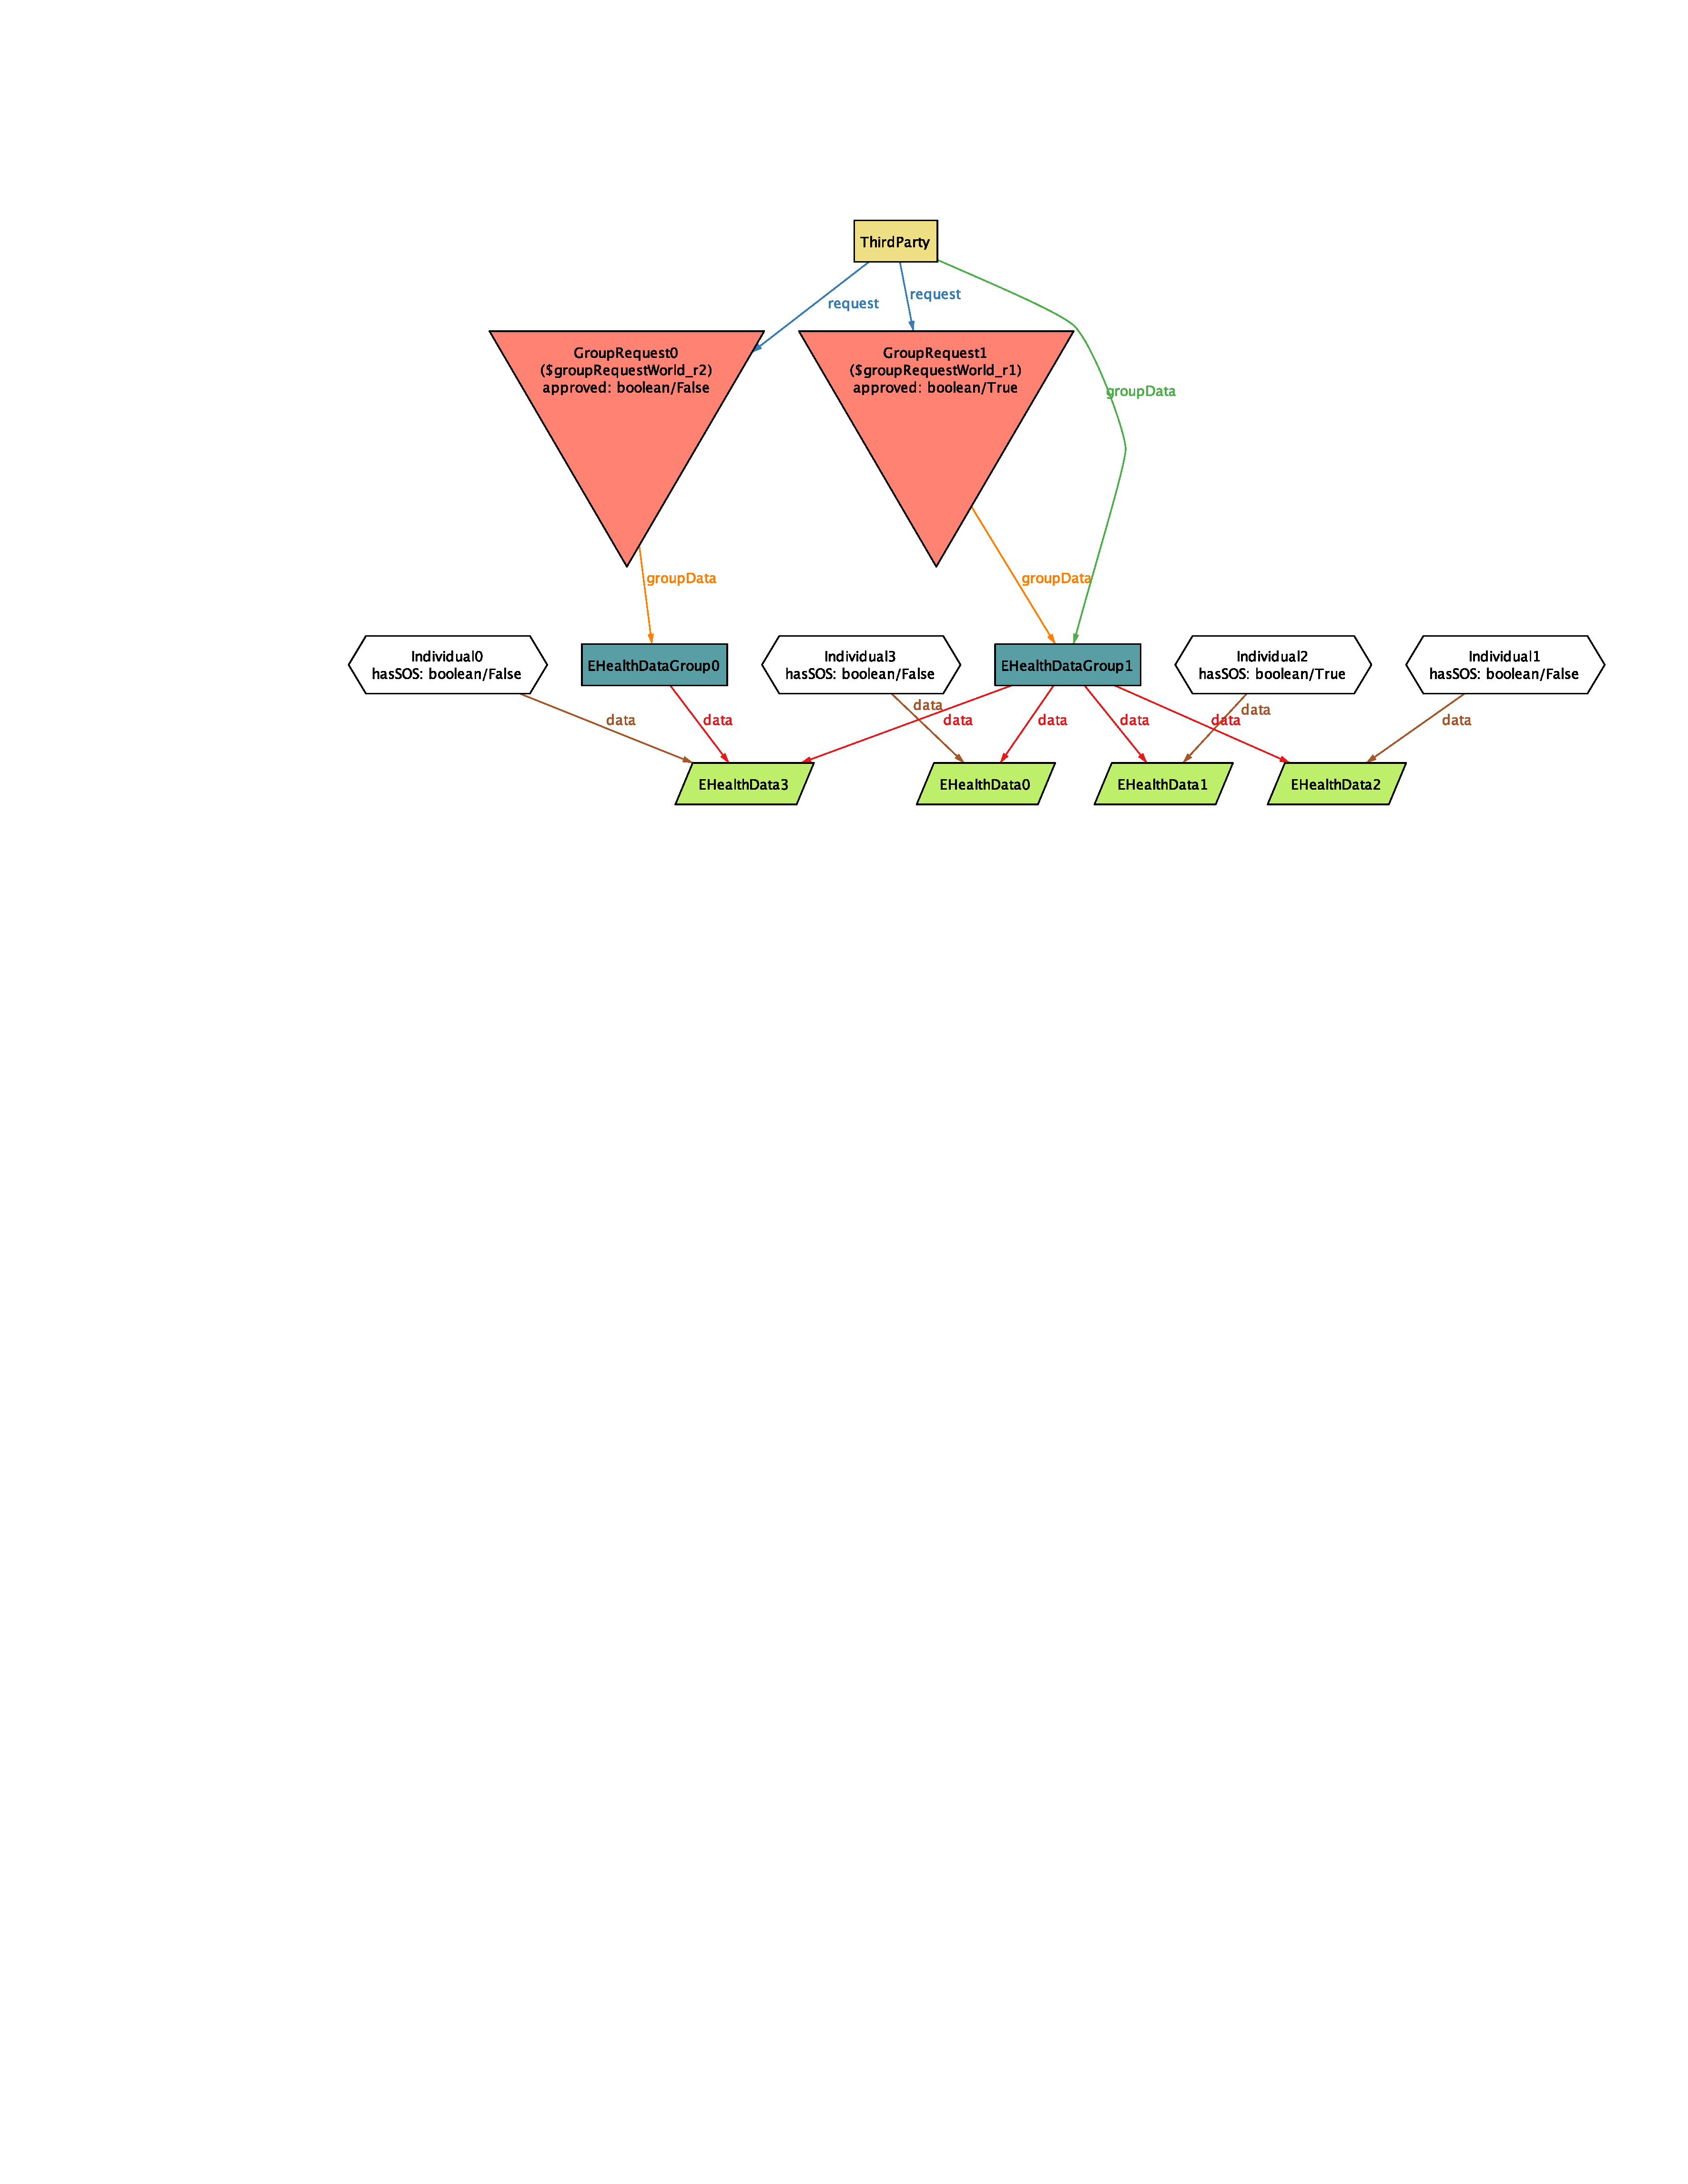
\includegraphics[scale=0.5, angle=-90]{resources/Alloy/group}}
\caption{World generated by \texttt{groupRequestWorld} predicate}\label{f:groupWorld}
\end{figure}

\section{Alloy results}
The checking of the four assertions defined in the model produce the results shown in Figure \ref{f:assertion}


\begin{figure}[H]
\centering
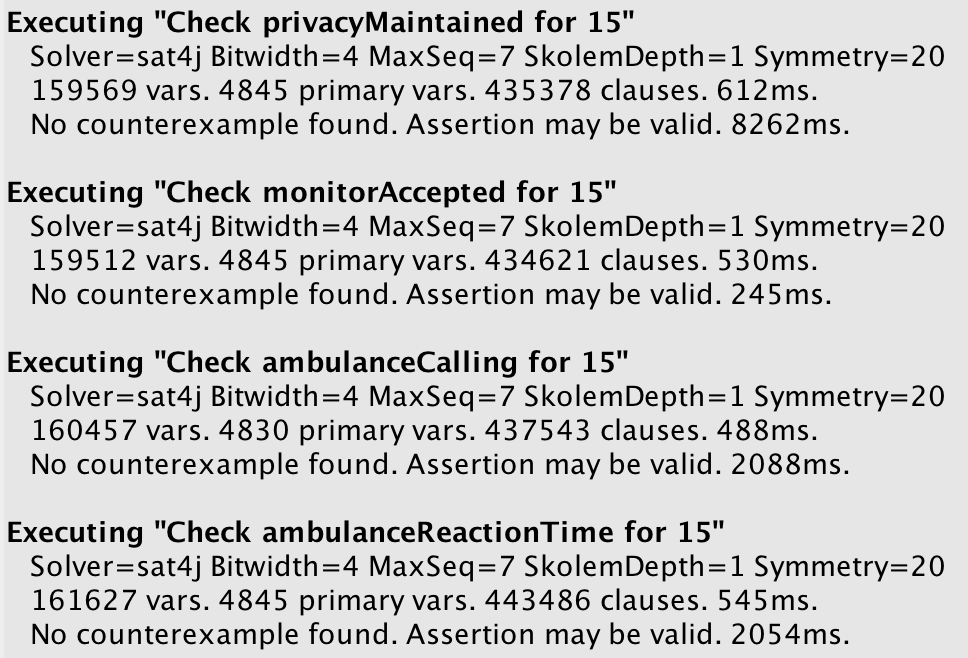
\includegraphics[scale=0.8]{resources/Alloy/assertion}
\caption{Checking of the four assertions}\label{f:assertion}
\end{figure}








\chapter{Effort spent}
In the following tables the time spent for each section of the project are presented, the specific requirements section is analyzed in details:

\renewcommand\arraystretch{1.5}
\begin{table}[ht]
\centering
\begin{tabular}{|l|l|}
\multicolumn{2}{c}{\textcolor{Blue}{\textbf{Stefano Pecchia}}} \\\hline
\multicolumn{1}{|c|}{\textbf{Section}} & \multicolumn{1}{|c|}{\textbf{Hours}} \\\hline
    Introduction & 6  
    \\ \hline
    Overall description & 4  
    \\ \hline 
    Exernal interfaces & 8  
     \\ \hline 
    Scenarios & 1  
       \\ \hline 
    Functional requirements & 8  
      \\ \hline 
      Non-functional requirements & 1
      \\ \hline
    Alloy & 1
	\\ \hline
	\end{tabular} \hspace{2.5em}
	\begin{tabular}{|l|l|}
\multicolumn{2}{c}{\textcolor{Blue}{\textbf{Edoardo Peretti}}} \\\hline
\multicolumn{1}{|c|}{\textbf{Task}} & \multicolumn{1}{|c|}{\textbf{Hours}} \\\hline
    Introduction & 1
    \\ \hline
    Overall description & 4  
    \\ \hline 
    Exernal interfaces & 0.5
     \\ \hline 
    Scenarios & 1  
       \\ \hline 
    Functional requirements & 2
      \\ \hline 
      Non-functional requirements & 0.5
    \\ \hline
    Alloy & 17
	\\ \hline
\end{tabular}
\end{table}
\chapter{References}

\begin{itemize}
\item Specification document "Mandatory Project Assignment AY 2018-2019.pdf"
\item ISO/IEC/IEEE 29148 - Standard on requirement engineering
\item WearOS by Google: https://wearos.google.com/\#hands-free-help
\item tool for building mockups: https://www.justinmind.com/
\item tool for uml diagrams: https://www.modelio.org/
\end{itemize}

\end{document}

